% MODIFICA EL CONTENIDO QUE VIENE A CONTINUACIÓN DE ACUERDO A TU TRABAJO

\chapter{Aprendizaje en Entornos Complejos}

%%%%%%%%%%%%%%%%%%%%%%%%%%%%%%%%%%%%%%%%%%%%%%%%%%%%%%%%%%%%%
%%%%%%%%%%%%%%%%%%%%%%%%%%%%%%%%%%%%%%%%%%%%%%%%%%%%%%%%%%%%%
\section{Introducción}

El aprendizaje por refuerzo representa una de las ramas más diversas de la inteligencia artificial, empleada para derrotar a campeones del mundo en juegos de mesa estratégicos o en la construcción de modelos de lenguaje avanzados. 
A diferencia del problema del bandido de $k$-brazos, donde las decisiones se toman en un entorno estático, los problemas del mundo real se desarrollan en un contexto dinámico. Cada decisión tomada por el agente modifica el estado del entorno, lo que requiere cálculos constantes para actualizar su percepción del mundo.

La motivación de este trabajo radica en comprender y aplicar algoritmos capaces de resolver tareas sin un conocimiento previo de la dinámica del entorno. Se pretende evolucionar desde los métodos tabulares clásicos, viables en espacios de estados reducidos, hasta el control con aproximaciones de función mediante redes neuronales, necesario para abordar entornos continuos y complejos.

Los objetivos principales de este informe son:
\begin{enumerate}
    \item Implementar y comparar el rendimiento de algoritmos de control tabular (Monte Carlo, SARSA y Q-Learning) en entornos de estados discretos.
    \item Desarrollar y evaluar algoritmos de control aproximado (Deep Q-Learning y SARSA semi-gradiente) en entornos continuos.
    \item Analizar el comportamiento, el rendimiento y la convergencia de los agentes basándose en la librería de gymnasium \cite{gymnasium} para llevar a cabo las pruebas.
\end{enumerate}

El documento se organiza de la siguiente manera: la sección de Desarrollo detalla el marco teórico necesario para aplicar los algoritmos de aprendizaje. La sección de Algoritmos expone el pseudocódigo y la lógica de los métodos implementados. Posteriormente, la Evaluación presenta los resultados empíricos obtenidos en los entornos seleccionados, y finalmente, se extraen las Conclusiones y líneas de mejora futuras.

%%%%%%%%%%%%%%%%%%%%%%%%%%%%%%%%%%%%%%%%%%%%%%%%%%%%%%%%%%%%%
%%%%%%%%%%%%%%%%%%%%%%%%%%%%%%%%%%%%%%%%%%%%%%%%%%%%%%%%%%%%%
\section{Desarrollo}

\subsection{Definición Formal del Problema}

El aprendizaje en entornos complejos se formaliza a través de un Proceso de Decisión de Markov (MDP). Un MDP se define mediante la tupla $\langle \mathcal{S}, \mathcal{A}, \mathcal{\{{P^a}\}_a}, \mathcal{R}, \gamma \rangle$, donde en cada instante $t$, el agente observa un estado $S_t \in \mathcal{S}$, ejecuta una acción $A_t \in \mathcal{A}$ siguiendo una política $\pi(a|s)$, y transita a un nuevo estado $S_{t+1}$ recibiendo una recompensa $R_{t+1}$.

\begin{definition}[Política]
Una política, representada como $\pi$, es una función que indica qué acción realizar de acuerdo al estado actual del entorno. Puede ser determinista, asignando una acción fija a un estado, o estocástica, proporcionando una distribución de probabilidad sobre las acciones posibles.
\end{definition}

El objetivo del agente es encontrar la política óptima $\pi^*$ que maximice el retorno esperado (la suma de recompensas descontadas a futuro):
\begin{equation}
    G_t = \sum_{k=0}^{\infty} \gamma^k R_{t+k+1}
\end{equation}

Para poder escoger la acción que lleve a un estado donde la recompensa sea máxima, el agente construye una representación interna del entorno basado en sus experiencias anteriores. La puntuación que asigna a cada estado el agente se basa en las ecuaciones de Bellman, que según el algoritmo implementado, se modifica para poder aplicar distintos enfoques. La fórmula general es la siguiente

\begin{equation}
    v(s) = \mathbb{E}[R_{t+1} + \gamma v(S_{t+1}) \mid S_t = s]
\end{equation}

Esta fórmula desglosa el valor de un estado en dos componentes principales:
\begin{itemize}
    \item \textbf{$R_{t+1}$:} Es la recompensa inmediata que el agente recibe al realizar una transición desde el estado actual $s$.
    \item \textbf{$\gamma v(S_{t+1})$:} Representa el valor del siguiente estado ($S_{t+1}$) multiplicado por el factor de descuento $\gamma$. Este factor determina la importancia de las recompensas futuras frente a las inmediatas.
\end{itemize}

Esta ecuación representa que el valor de un estado es la recompensa inmediata más un valor a futuro, que representa el pasar a un próximo estado.

Para aplicar esta ecuación a cierto problema, se necesitan datos que involucren la obtención de recompensas.
\begin{definition}[Episodio]
Un episodio se define como una secuencia que involucra pasar por un estado, tomar una acción y obtener una recompensa por alcanzar otro estado, terminando el episodio en un estado terminal teoricamente. En tareas episódicas, el agente utiliza la retroalimentación obtenida al final o durante el transcurso del episodio para maximizar la recompensa acumulativa futura
\end{definition}

\subsection{Enfoques y Métodos Utilizados}

Cuando no se conoce el modelo de transiciones $\mathcal{P}$ ni la función de recompensa $\mathcal{R}$, el agente debe aprender a través de la experiencia. El objetivo que tiene este es actualizar su representación del entorno (tabla de estados-acciones $Q$) para poder elegir, dado un estado $S$, la acción $A$ que maximice su retorno. Las familias de métodos estudiadas se muestran a continuación por antigüedad.

\begin{itemize}
    \item \textbf{Métodos de Monte Carlo (MC):} Requieren que el episodio termine para calcular el retorno real $G_t$ y actualizar el valor de los estados visitados. Son métodos de alta varianza pero sin sesgo.
    \item \textbf{Métodos de Diferencias Temporales (TD):} Combinan ideas de MC y Programación Dinámica. Actualizan las estimaciones basándose en otras estimaciones parciales (bootstrapping) paso a paso, sin esperar al final del episodio.
    \item \textbf{Control con Aproximaciones:} Cuando el espacio de estados es inmenso o continuo, es imposible mantener una tabla $Q(s,a)$. Se opta por aproximar la función de valor como una forma funcional parametrizada con un vector de pesos.
\end{itemize}

Estos enfoques mejoran gradualmente la aplicabilidad del agente. Los métodos TD mejoran a MC en entornos largos o continuos al aprender paso a paso, mientras que los métodos aproximados (DQN) suponen el salto cualitativo definitivo para resolver tareas complejas inabarcables mediante técnicas tabulares. 

Aunque los últimos métodos mencionados sean los más complejos, en \cite{qlearningtrafico} se utilizó Q-Learning con ciertas optimizaciones para la optimización del movimiento de aeronaves en tierra dentro de los aeropuertos, demostrando ser más eficiente que los métodos tradicionales. Otro ejemplo conocido que usaba métodos aproximados es el de \cite{atariDQN}, donde se usó Deep Q-Learning para conseguir resultados propios del estado del arte en cuanto a rendimiento en juegos de la consola Atari 2600, introduciendo únicamente píxeles como input a la red.

Este trabajo se diferencia de otros enfoques previos al alejarse de la mera réplica de tutoriales para establecer y seguir un criterio de evaluación y una metodología propia.

%%%%%%%%%%%%%%%%%%%%%%%%%%%%%%%%%%%%%%%%%%%%%%%%%%%%%%%%%%%%%
%%%%%%%%%%%%%%%%%%%%%%%%%%%%%%%%%%%%%%%%%%%%%%%%%%%%%%%%%%%%%
\section{Algoritmos}

A continuación, se describen los algoritmos estudiados. Todos los agentes siguen la misma interfaz estructural basada en los métodos \texttt{get\_action(obs)} y \texttt{update(...)} típica de gymnasium.

\subsection*{Monte Carlo Control (Off-policy)}
Este algoritmo separa la política que se está aprendiendo (objetivo, $\pi$) de la política que genera el comportamiento (comportamiento o behavior, $b$), permitiendo aprender una política determinista óptima a partir de datos generados por una política exploratoria $\varepsilon$-soft. La diferencia entre las dos políticas se corrige mediante muestreo por importancia ponderado.

\begin{algorithm}
\caption{Control de Monte Carlo (off-policy)}\label{algo:mc_off_policy}
\begin{algorithmic}[1]
\State \textbf{Inicializar, para todo $s \in \mathcal{S}, a \in \mathcal{A}(s)$:}
    \State $Q(s, a) \in \mathbb{R}$ (arbitrariamente)
    \State $C(s, a) \gets 0$
    \State $\pi(s) \gets \arg\max_a Q(s, a)$ \Comment{con empates rotos consistentemente}
\State \textbf{Repetir para siempre (para cada episodio):}
    \State $b \gets$ cualquier política blanda (\textit{soft policy})
    \State Generar un episodio usando $b$: $S_0, A_0, R_1, \dots, S_{T-1}, A_{T-1}, R_T$
    \State $G \gets 0$
    \State $W \gets 1$
    \For{$t = T-1, T-2, \dots, 0$}
        \State $G \gets \gamma G + R_{t+1}$
        \State $C(S_t, A_t) \gets C(S_t, A_t) + W$
        \State $Q(S_t, A_t) \gets Q(S_t, A_t) + \dfrac{W}{C(S_t, A_t)} \bigl[ G - Q(S_t, A_t) \bigr]$
        \State $\pi(S_t) \gets \arg\max_a Q(S_t, a)$ \Comment{con empates rotos consistentemente}
        \If{$A_t \neq \pi(S_t)$} 
            \State \textbf{salir del bucle interno} \Comment{proceder al siguiente episodio}
        \EndIf
        \State $W \gets W \dfrac{1}{b(A_t|S_t)}$
    \EndFor
\end{algorithmic}
\end{algorithm}

A pesar de que en la práctica los algoritmos de diferencias temporales suelen ser más eficientes, el concepto de Monte Carlo se aplica en algoritmos más complejos como REINFORCE que se basa en el gradiente de política.

\subsection*{Monte Carlo Control First-Visit (On-policy)}
Este algoritmo es un caso concreto del anterior, donde la política de comportamiento y la política objetivo son la misma. Además solo se actualiza un par (estado,valor) la primera vez que aparece en un episodio.

\subsection*{Sarsa (on-policy TD control)}
A diferencia de los métodos de Monte Carlo, Sarsa es un algoritmo de Diferencias Temporales (TD) que actualiza la tabla de valores $Q$ cada paso (con TD(0)). Es un método on-policy ya que utiliza la misma política para obtener la próxima acción del agente, necesaria para calcular el valor esperado del estado actual.

\begin{algorithm}[h]
\caption{Sarsa: Control TD en la política (on-policy) para estimar $Q \approx q_*$}\label{algo:sarsa}
\begin{algorithmic}[1]
\Require Parámetros del algoritmo: tamaño de paso $\alpha \in (0, 1]$, $\varepsilon > 0$ pequeño
\State Inicializar $Q(s, a)$, para todo $s \in \mathcal{S}^+, a \in \mathcal{A}(s)$, arbitrariamente excepto que $Q(terminal, \cdot) = 0$
\For{cada episodio}
    \State Inicializar $S$
    \State Elegir $A$ desde $S$ usando una política derivada de $Q$ (p.e., $\varepsilon$-greedy)
    \While{$S$ no sea terminal}
        \State Realizar la acción $A$, observar $R$ y el siguiente estado $S'$
        \State Elegir $A'$ desde $S'$ usando una política derivada de $Q$ (p.e., $\varepsilon$-greedy)
        \State $Q(S, A) \gets Q(S, A) + \alpha \bigl[ R + \gamma Q(S', A') - Q(S, A) \bigr]$
        \State $S \gets S'$
        \State $A \gets A'$
    \EndWhile
\EndFor
\end{algorithmic}
\end{algorithm}
SARSA es un algoritmo que toma en cuenta sus decisiones en el futuro, por lo que su política se vuelve más conservadora.

\subsection*{Q-Learning (off-policy TD control)}
Este es un método off-policy que actualiza $Q(S, A)$ asumiendo que en el siguiente estado se tomará la acción óptima ($\max_a Q(S', a)$), incluso si el agente termina realizando una acción diferente por exploración.
\begin{algorithm}[!h]
\caption{Q-learning: Control TD fuera de la política (off-policy) para estimar $\pi \approx \pi_*$}\label{algo:q_learning_tabular}
\begin{algorithmic}[1]
\Require Parámetros del algoritmo: tamaño de paso $\alpha \in (0, 1]$, $\varepsilon > 0$ pequeño
\State Inicializar $Q(s, a)$, para todo $s \in \mathcal{S}^+, a \in \mathcal{A}(s)$, arbitrariamente excepto que $Q(terminal, \cdot) = 0$
\For{cada episodio}
    \State Inicializar $S$
    \Repeat \Comment{Para cada paso del episodio}
        \State Elegir $A$ desde $S$ usando una política derivada de $Q$ (p.e., $\varepsilon$-greedy)
        \State Realizar la acción $A$, observar $R$ y el siguiente estado $S'$
        \State $Q(S, A) \gets Q(S, A) + \alpha \bigl[ R + \gamma \max_a Q(S', a) - Q(S, A) \bigr]$
        \State $S \gets S'$
    \Until{$S$ es terminal}
\EndFor
\end{algorithmic}
\end{algorithm}
Q-Learning, al ser off-policy, se aproxima más a la política óptima que SARSA debido a que su política objetivo es greedy y siempre escoge el estado con máximo valor.

\subsection*{Sarsa semi-gradiente episódico}
A diferencia de los métodos tabulares, SARSA semi-gradiente utiliza una función de valor de acción parametrizada ($\hat{q}$) y actualiza un vector de pesos ($\mathbf{w}$) mediante descenso de gradiente para generalizar el aprendizaje en espacios de estados grandes o continuos.
\begin{algorithm}[!h]
\caption{Sarsa semi-gradiente episódico para estimar $\hat{q} \approx q_*$}\label{algo:semi_gradient_sarsa}
\begin{algorithmic}[1]
\State \textbf{Entrada:} una parametrización de función de valor de acción diferenciable $\hat{q} : \mathcal{S} \times \mathcal{A} \times \mathbb{R}^d \to \mathbb{R}$
\Require tamaño de paso $\alpha > 0$, $\varepsilon > 0$ pequeño
\State Inicializar los pesos de la función de valor $\mathbf{w} \in \mathbb{R}^d$ arbitrariamente (p.e., $\mathbf{w} = \mathbf{0}$)
\For{cada episodio}
    \State $S, A \gets$ estado y acción inicial del episodio (p.e., $\varepsilon$-greedy)
    \While{$S$ no sea terminal}
        \State Realizar la acción $A$, observar $R$ y el siguiente estado $S'$
        \If{$S'$ es terminal}
            \State $\mathbf{w} \gets \mathbf{w} + \alpha \bigl[ R - \hat{q}(S, A, \mathbf{w}) \bigr] \nabla \hat{q}(S, A, \mathbf{w})$
            \State \textbf{ir al siguiente episodio}
        \EndIf
        \State Elegir $A'$ como una función de $\hat{q}(S', \cdot, \mathbf{w})$ (p.e., $\varepsilon$-greedy)
        \State $\mathbf{w} \gets \mathbf{w} + \alpha \bigl[ R + \gamma \hat{q}(S', A', \mathbf{w}) - \hat{q}(S, A, \mathbf{w}) \bigr] \nabla \hat{q}(S, A, \mathbf{w})$
        \State $S \gets S'$
        \State $A \gets A'$
    \EndWhile
\EndFor
\end{algorithmic}
\end{algorithm}

Este algoritmo permite manejar espacios de estado enormes o continuos al no depender de una tabla de valores $Q$.

\subsection*{Deep Q-Learning (DQN) con Experience Replay}
DQN extiende Q-Learning aproximando $q(s,a)$ con una red neuronal profunda $\hat{q}(s,a;\mathbf{w})$ que recibe el estado como entrada y devuelve los valores de todas las acciones posibles. Para estabilizar el aprendizaje utiliza \textit{Experience Replay} (muestreo aleatorio de transiciones almacenadas) y una \textit{Target Network} con parámetros congelados $\mathbf{w}^-$ que reduce la oscilación del target.

\begin{algorithm}[!h]
\caption{Deep Q-Learning con Experience Replay}\label{algo:dqn}
\begin{algorithmic}[1]
\State Inicializar memoria de repetición $D$ con capacidad $N$
\State Inicializar red $Q$ con pesos aleatorios $\mathbf{w}$
\State Inicializar red objetivo con $\mathbf{w}^- \gets \mathbf{w}$
\For{cada episodio}
    \State Inicializar estado $s_1$
    \For{$t=1$ hasta $T$}
        \State Con probabilidad $\epsilon$ elegir acción aleatoria; si no, $a_t=\arg\max_a \hat{q}(s_t,a;\mathbf{w})$
        \State Ejecutar $a_t$, observar $r_t$, $s_{t+1}$ y $done$
        \State Guardar $(s_t,a_t,r_t,s_{t+1},done)$ en $D$
        \State Muestrear un minibatch aleatorio de $D$
        \For{cada transición $(s_j,a_j,r_j,s_{j+1},done_j)$}
            \If{$done_j$}
                \State $y_j \gets r_j$
            \Else
                \State $y_j \gets r_j + \gamma \max_{a'} \hat{q}(s_{j+1},a';\mathbf{w}^-)$
            \EndIf
        \EndFor
        \State Actualizar $\mathbf{w}$ con un paso de gradiente sobre $(y_j-\hat{q}(s_j,a_j;\mathbf{w}))^2$
        \State Cada $C$ pasos: $\mathbf{w}^- \gets \mathbf{w}$
    \EndFor
\EndFor
\end{algorithmic}
\end{algorithm}

DQN es off-policy y permite escalar Q-Learning a espacios de estados continuos o de alta dimensión, manteniendo el control mediante una política $\epsilon$-greedy sobre la red.
%%%%%%%%%%%%%%%%%%%%%%%%%%%%%%%%%%%%%%%%%%%%%%%%%%%%%%%%%%%%%
%%%%%%%%%%%%%%%%%%%%%%%%%%%%%%%%%%%%%%%%%%%%%%%%%%%%%%%%%%%%%
\section{Evaluación/Experimentos}

\subsection{Configuración Experimental}

Las pruebas se realizaron con la librería Gymnasium y semilla fija (SEED=2024) para garantizar reproducibilidad. Se estudiaron tres entornos representativos:

\begin{itemize}
    \item \textbf{Taxi-v3 (discreto):} 500 estados, 6 acciones. Recompensas: $-1$ por paso, $+20$ entrega exitosa, $-10$ acción ilegal. Entrenamiento de 100\,000 episodios para comparar MC, SARSA y Q-Learning.
    \item \textbf{CliffWalking-v1 (discreto):} grid 4$\times$12 (48 estados), 4 acciones. Recompensas: $-1$ por paso, $-100$ caída al acantilado y $0$ al llegar. Entrenamiento de 10\,000 episodios para comparar Q-Learning vs SARSA.
    \item \textbf{LunarLander-v3 (continuo):} estado de 8 variables continuas y 4 acciones discretas: $0$ (no hacer nada), $1$ (motor lateral izquierdo), $2$ (motor principal), $3$ (motor lateral derecho). Elegimos el espacio de acciones discreto porque DQN y SARSA-SG están formulados para acciones discretas; usar el espacio continuo exigiría métodos de política/actor-crítico (p.ej., DDPG/PPO). Entrenamiento de 5\,000 episodios para DQN y SARSA semi-gradiente.
\end{itemize}

Parámetros base utilizados:

\begin{itemize}
    \item \textbf{Tabulares (Taxi):} $\epsilon$-greedy con decaimiento $\epsilon_t=\min(1,1000/(t+1))$, $\alpha=0.1$, $\gamma=1.0$.
    \item \textbf{Tabulares (Cliff):} $\epsilon$-greedy con el mismo decaimiento, $\alpha=0.1$, $\gamma=0.99$.
    \item \textbf{DQN (base):} $\alpha=0.0005$, $\gamma=0.99$, buffer 50k, batch 64, target update $C=2000$, red 64$\times$64, $\epsilon$ decay $0.999$ (mínimo 0.01).
    \item \textbf{SARSA-SG (base):} $\alpha=0.001$, $\gamma=0.99$, red 64$\times$64, $\epsilon$ decay $0.995$ (mínimo 0.01).
\end{itemize}

\subsection{Métricas}

Para evaluar el aprendizaje se midieron tres indicadores:
\begin{itemize}
    \item \textbf{Recompensa media acumulada por episodio}: $\bar{R}_t = \frac{1}{t}\sum_{i=1}^{t} R_i$. En entornos con fuertes penalizaciones iniciales (CliffWalking) esta métrica puede permanecer muy negativa.
    \item \textbf{Longitud media de episodios}: número de pasos por episodio (se reporta la media de los últimos 1000 episodios).
    \item \textbf{Pérdida (solo DQN)}: evolución de la loss Huber para analizar estabilidad del entrenamiento.
\end{itemize}

\subsection{Resultados y Análisis Crítico}

\subsubsection*{Taxi-v3 (control tabular)}
Como se aprecia en la Figura~\ref{fig:taxi-recompensa}, la comparación conjunta (misma configuración de hiperparámetros) confirma que los métodos TD superan claramente a Monte Carlo en velocidad de convergencia.

\begin{table}[h]
\centering
\resizebox{\columnwidth}{!}{%
\begin{tabular}{lcc}
\hline
\textbf{Algoritmo} & \textbf{Recompensa media final} & \textbf{Longitud media final (pasos)} \\
\hline
MC On-Policy & -138.82 & 113.73 \\
MC Off-Policy & -22.32 & 13.69 \\
SARSA & -5.34 & 13.04 \\
Q-Learning & -4.47 & 13.06 \\
\hline
\end{tabular}%
}
\caption{Resultados en Taxi-v3 (100k episodios).}
\end{table}

Los métodos TD convergen en pocos miles de episodios, mientras que MC on-policy queda anclado en episodios largos, como se ve en la Figura~\ref{fig:taxi-pasos}. Q-Learning y SARSA terminan prácticamente empatados en Taxi-v3 (recompensa -4.47 vs -5.34 y longitud 13.06 vs 13.04), lo que indica que en este entorno la diferencia on/off-policy apenas se nota; la dinámica no penaliza de forma fuerte la exploración. Por eso, para analizar con más claridad esa diferencia, se evalúa después CliffWalking, donde el riesgo de caer introduce un contraste real entre ambos métodos. En Q-Learning, un $\epsilon$ fijo muy bajo (0.01) da recompensas positivas (6.31), mientras que $\gamma=0.05$ no aprende (longitud media 82.97 pasos) porque el descuento es tan fuerte que la recompensa final no se propaga hacia atrás, tal como muestran las curvas de la Figura~\ref{fig:taxi-qlearn-hypers}. En SARSA ocurre algo similar: $\epsilon=0.01$ mejora el rendimiento (recompensa 6.26, 13.25 pasos) y $\gamma=0.25$ lo degrada claramente (recompensa -159.61, 112.51 pasos) al reducir demasiado la importancia del retorno futuro, visible en la Figura~\ref{fig:taxi-sarsa-hypers}.

\begin{figure}[!htbp]
    \centering
    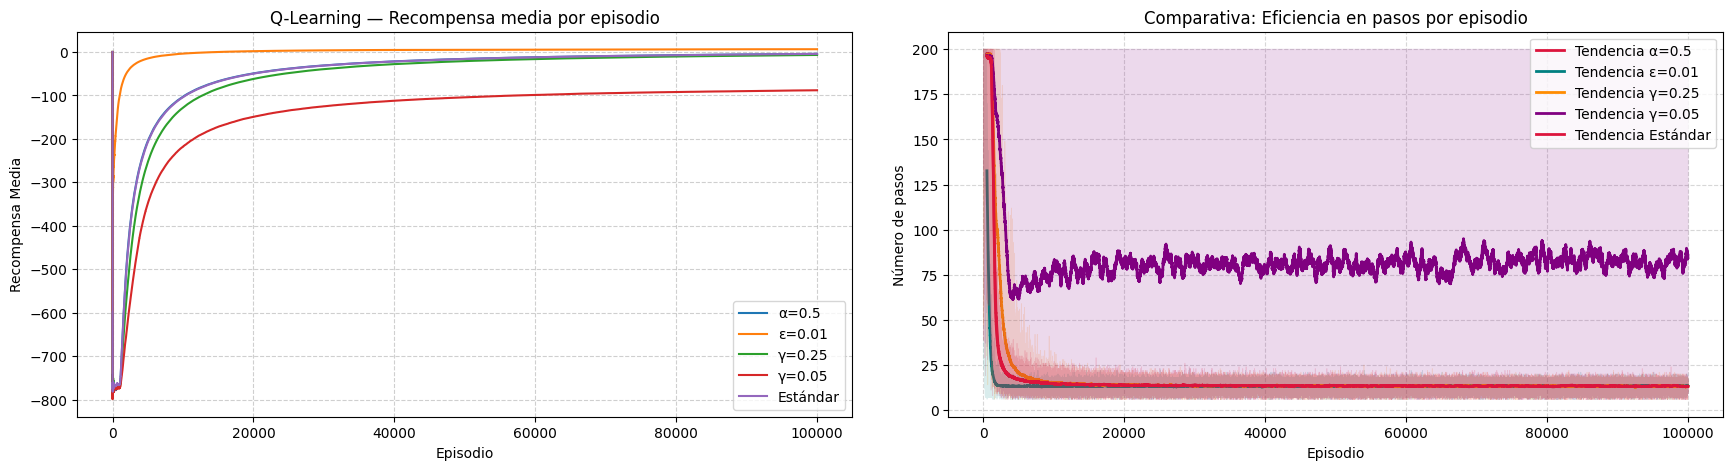
\includegraphics[width=0.95\linewidth]{imagenes/taxi_qlearning_hyper_combo.png}
    \caption{Taxi-v3: Q-Learning con variaciones de $\alpha$, $\epsilon$ y $\gamma$.}
    \label{fig:taxi-qlearn-hypers}
\end{figure}

\begin{figure}[!htbp]
    \centering
    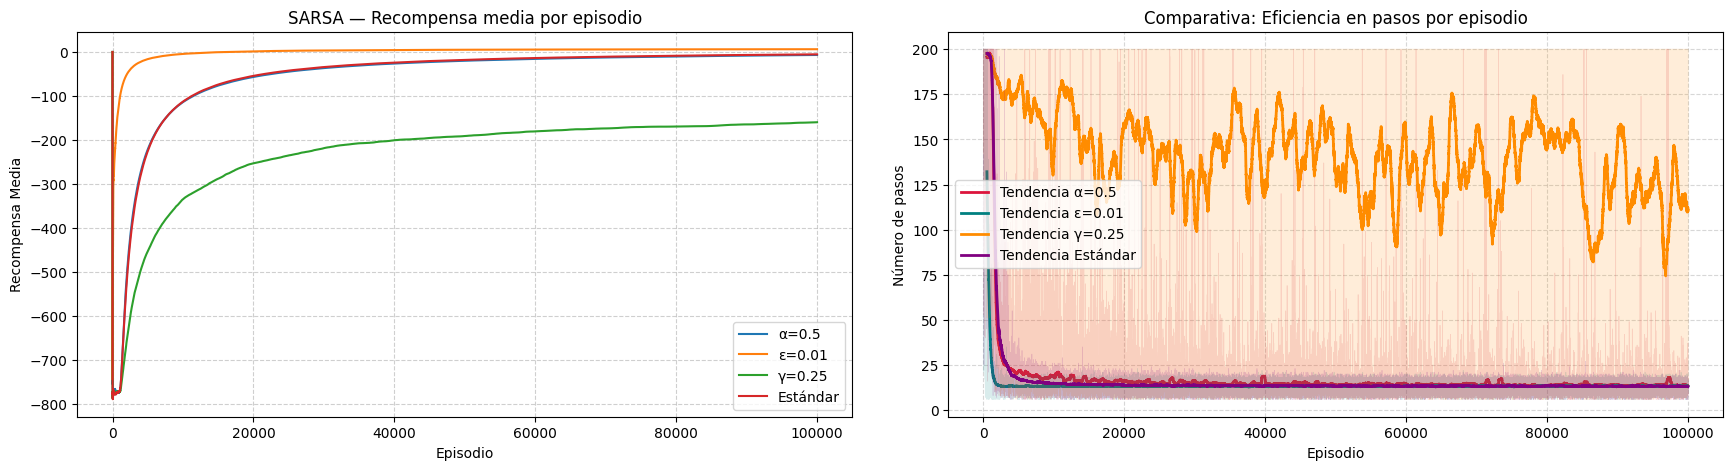
\includegraphics[width=0.95\linewidth]{imagenes/taxi_sarsa_hyper_combo.png}
    \caption{Taxi-v3: SARSA con variaciones de $\alpha$, $\epsilon$ y $\gamma$.}
    \label{fig:taxi-sarsa-hypers}
\end{figure}

La diferencia entre MC on-policy y off-policy es clara: con on-policy el agente mantiene mucha exploración y los episodios permanecen largos, mientras que off-policy puede seguir una política objetivo más greedy y reduce rápidamente la longitud. Esto se aprecia en la Figura~\ref{fig:taxi-pasos}, donde MC on-policy se estabiliza alrededor de 110–120 pasos, y MC off-policy cae a valores cercanos a 14–15 pasos, alineados con SARSA y Q-Learning.

\begin{figure}[!htbp]
    \centering
    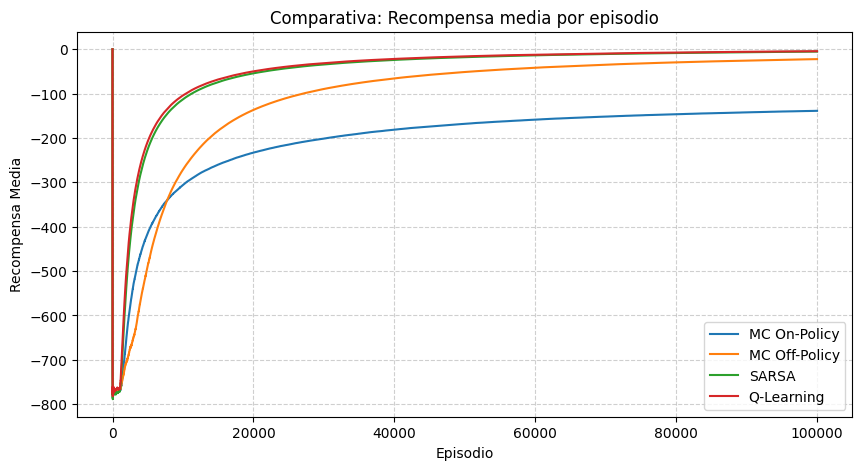
\includegraphics[width=0.9\linewidth]{imagenes/taxi_comparativa_recompensa.png}
    \caption{Taxi-v3: recompensa media por episodio (MC on/off, SARSA y Q-Learning).}
    \label{fig:taxi-recompensa}
\end{figure}

\begin{figure}[!htbp]
    \centering
    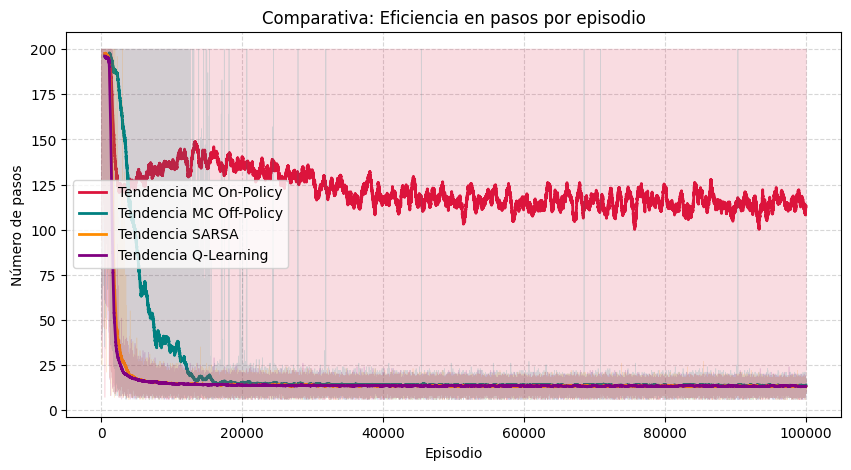
\includegraphics[width=0.9\linewidth]{imagenes/taxi_comparativa_pasos.png}
    \caption{Taxi-v3: eficiencia en pasos por episodio (tendencias suavizadas).}
    \label{fig:taxi-pasos}
\end{figure}

\subsubsection*{CliffWalking-v1 (riesgo vs optimalidad)}
Aquí se observa la diferencia on-policy/off-policy. Q-Learning converge a la ruta óptima (13 pasos) en el episodio greedy, mientras SARSA aprende la ruta segura (17 pasos) porque, al ser on-policy, internaliza el riesgo de sus propias acciones exploratorias. La media acumulada refleja muchas caídas iniciales porque al explorar el agente cae con frecuencia al acantilado y recibe una penalización fuerte (-100), lo que mantiene la media muy negativa durante los primeros miles de episodios (Figura~\ref{fig:cliff-recompensa}):

\begin{itemize}
    \item Q-Learning: recompensa media final -6845.23, longitud media 17.08 pasos.
    \item SARSA: recompensa media final -8025.64, longitud media 19.33 pasos.
\end{itemize}

Con $\epsilon=0.01$ ambos mejoran notablemente: Q-Learning se acerca a 13.36 pasos y SARSA a 15.19 pasos. En Q-Learning, $\gamma=0.05$ falla (longitud media $>180$ pasos). La eficiencia en pasos durante el entrenamiento se compara en la Figura~\ref{fig:cliff-pasos}.

\begin{figure}[!htbp]
    \centering
    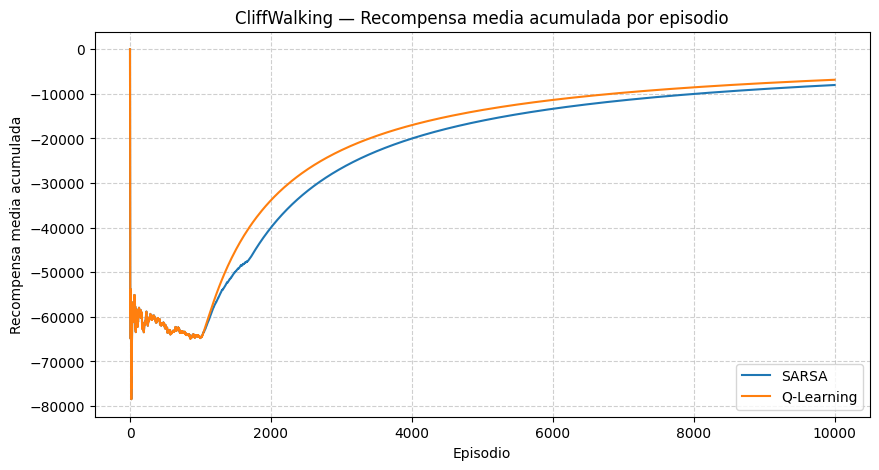
\includegraphics[width=0.9\linewidth]{imagenes/cliff_comparativa_recompensa.png}
    \caption{CliffWalking-v1: recompensa media acumulada por episodio (SARSA vs Q-Learning).}
    \label{fig:cliff-recompensa}
\end{figure}

\begin{figure}[!htbp]
    \centering
    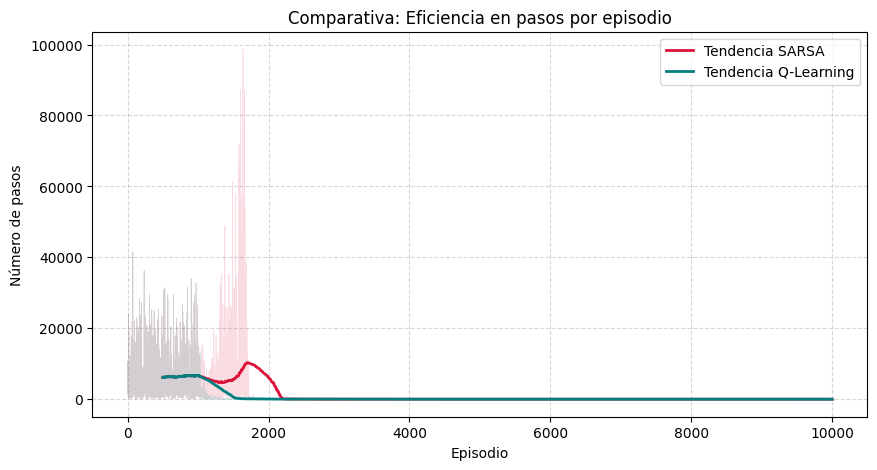
\includegraphics[width=0.9\linewidth]{imagenes/cliff_comparativa_pasos.png}
    \caption{CliffWalking-v1: eficiencia en pasos por episodio (SARSA vs Q-Learning).}
    \label{fig:cliff-pasos}
\end{figure}

\subsubsection*{LunarLander-v3 (control aproximado)}
En el entorno continuo se requiere aproximación de función. Con los hiperparámetros base, SARSA-SG alcanza recompensa superior pero DQN obtiene episodios más cortos:

\begin{itemize}
    \item SARSA-SG (base 64x64): recompensa media final 176.38, longitud media 295.29 pasos.
    \item DQN (base): recompensa media final 118.11, longitud media 206.23 pasos.
\end{itemize}

La sensibilidad de DQN a sus hiperparámetros es clara: con $C=50$ la recompensa cae a -493.42, mientras que $C=10000$ mejora ligeramente (129.99), como se ve en la Figura~\ref{fig:lunar-dqn-target}. En el barrido del buffer (Figura~\ref{fig:lunar-dqn-buffer}), la configuración base (50k) ronda 118 puntos, pero al reducirlo a 5k baja a 51.47 y con 1k se desploma a 18.60, evidenciando la necesidad de decorrelación temporal.

En SARSA-SG, el barrido de arquitectura también muestra diferencias: una red 128$\times$128 alcanza 173.93 con 265.23 pasos, mientras que una 16$\times$16 cae a 106.02 y 417.75 pasos, confirmando que la capacidad de la función aproximadora es crítica en LunarLander (Figura~\ref{fig:lunar-sarsa-arch}). La comparación directa entre ambos métodos se muestra en las Figuras~\ref{fig:lunar-comp-recompensa} y~\ref{fig:lunar-comp-pasos}.

\begin{figure}[!htbp]
    \centering
    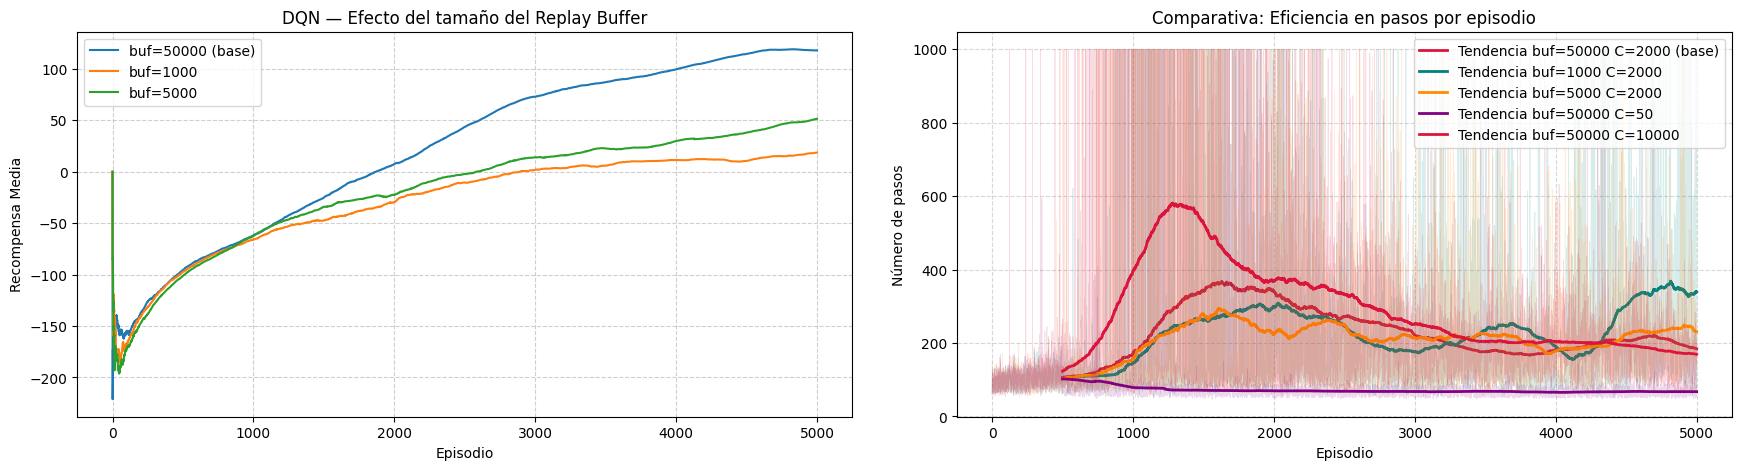
\includegraphics[width=0.95\linewidth]{imagenes/lunar_dqn_buffer_combo.png}
    \caption{LunarLander-v3: DQN — efecto del tamaño del Replay Buffer.}
    \label{fig:lunar-dqn-buffer}
\end{figure}

\begin{figure}[!htbp]
    \centering
    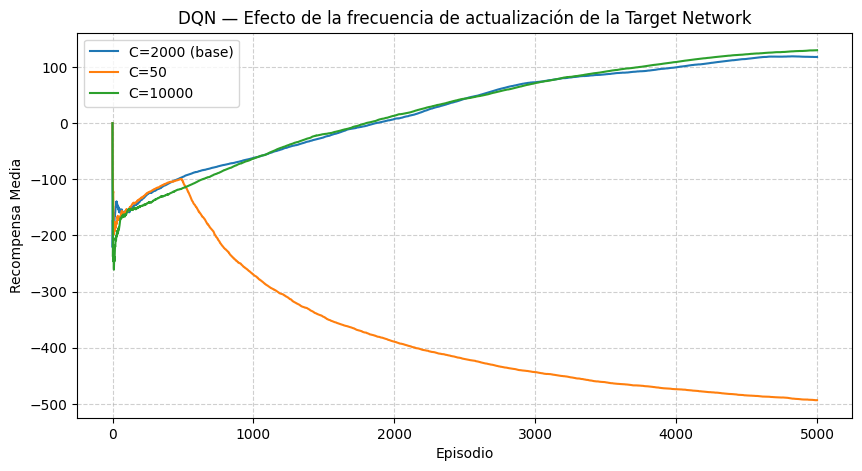
\includegraphics[width=0.9\linewidth]{imagenes/lunar_dqn_target_recompensa.png}
    \caption{LunarLander-v3: DQN — efecto de la frecuencia de actualización de la Target Network ($C$).}
    \label{fig:lunar-dqn-target}
\end{figure}

\begin{figure}[!htbp]
    \centering
    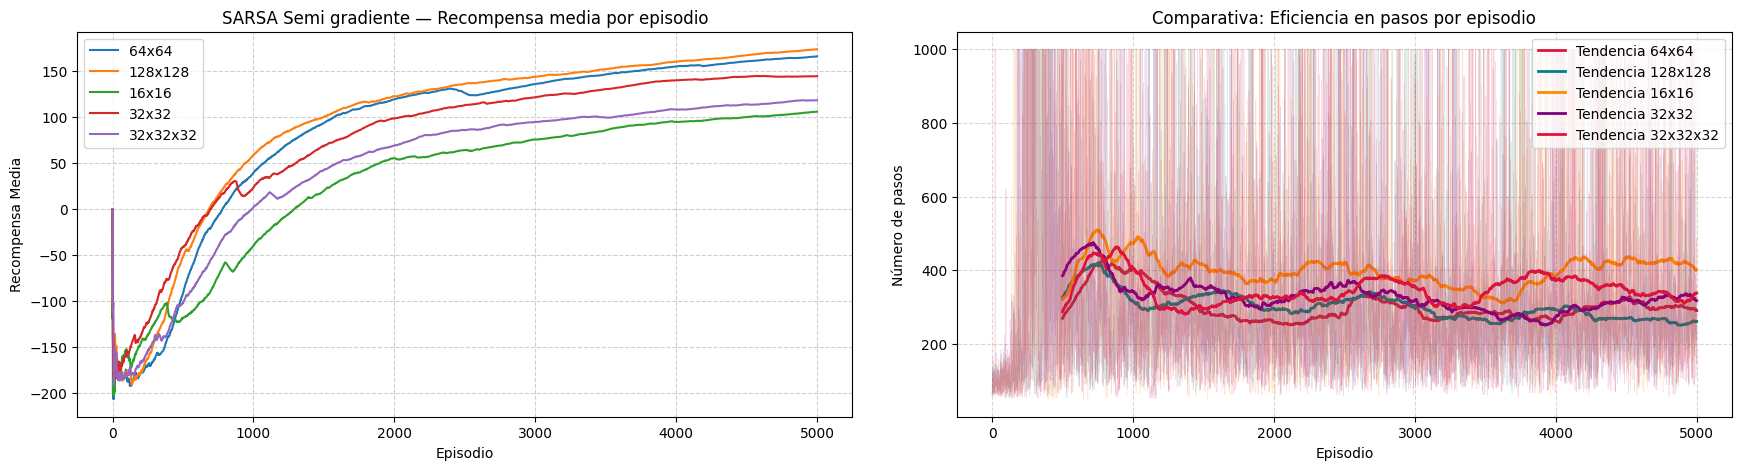
\includegraphics[width=0.95\linewidth]{imagenes/lunar_sarsa_sg_arch_combo.png}
    \caption{LunarLander-v3: SARSA-SG — efecto de la arquitectura de red.}
    \label{fig:lunar-sarsa-arch}
\end{figure}

\begin{figure}[!htbp]
    \centering
    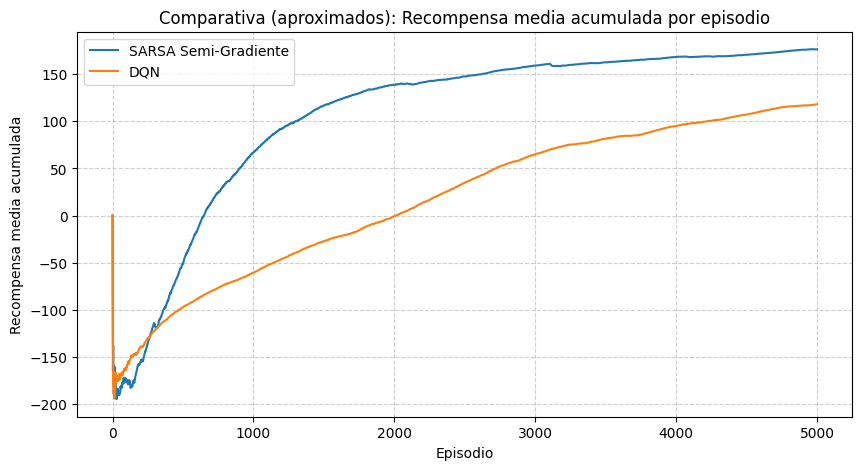
\includegraphics[width=0.9\linewidth]{imagenes/lunar_comparativa_recompensa.png}
    \caption{LunarLander-v3: recompensa media acumulada por episodio (SARSA-SG vs DQN).}
    \label{fig:lunar-comp-recompensa}
\end{figure}

\begin{figure}[!htbp]
    \centering
    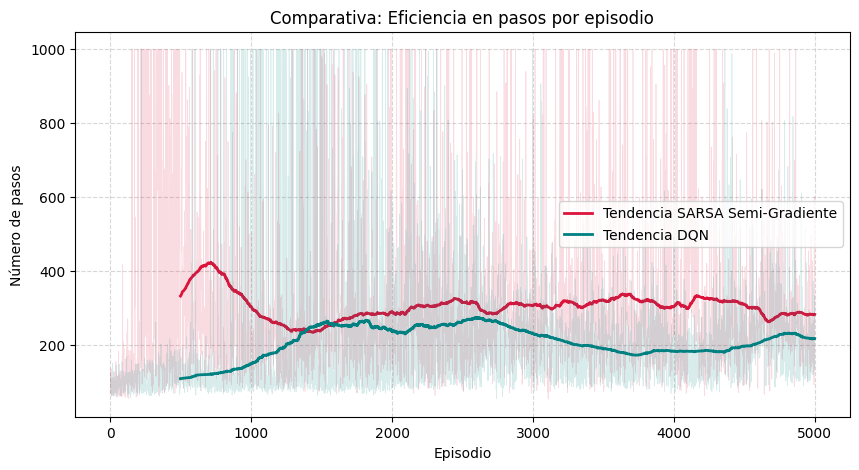
\includegraphics[width=0.9\linewidth]{imagenes/lunar_comparativa_pasos.png}
    \caption{LunarLander-v3: eficiencia en pasos por episodio (SARSA-SG vs DQN).}
    \label{fig:lunar-comp-pasos}
\end{figure}

\section{Conclusiones}

Los resultados permiten extraer varias conclusiones:
\begin{itemize}
    \item En entornos discretos largos (Taxi-v3), los métodos TD superan ampliamente a Monte Carlo por su bootstrapping paso a paso.
    \item La dimensión on-policy/off-policy es crítica en CliffWalking: SARSA aprende rutas seguras y Q-Learning tiende a la ruta óptima aunque explore con riesgo.
    \item En entornos continuos, la aproximación con redes es imprescindible. DQN es estable pero sensible a $C$ y al tamaño del buffer; SARSA-SG puede rendir mejor con una tasa de aprendizaje mayor.
    \item La comparación DQN vs SARSA-SG no es absoluta: el ranking depende de hiperparámetros y horizonte de entrenamiento.
\end{itemize}

Como trabajo futuro se propone repetir con múltiples semillas, igualar hiperparámetros entre aproximadores y evaluar variantes como Double DQN o Prioritized Replay.
